\chapter{An improved framework for downscaling cloud properties from
large-scale models}\label{sec:subgrid2}

The previous chapter identified errors in simulated satellite cloud
diagnostics that arise from using unrealistic cloud overlap assumptions
and horizontally homogeneous condensate. In this chapter, an improved
subcolumn generator is presented, building on the work of previous
investigators, to reduce those errors and enable more consistent and
robust comparisons of modeled and satellite-retrieved cloud statistics.

The improved subcolumn generator described here uses a scheme developed
by \citet{raisanen_et_al_2004} to generate subcolumn cloud condensate
that both follows a more realistic and flexible cloud overlap assumption
and allows for generating subcolumn condensate with horizontal
variability. This scheme has been extended here to apply to
precipitation as well. Using the same framework as in
Section~\ref{sec:subgrid1}, the new subcolumn generator presented here
is shown to substantially reduced the identified errors that arise in
using SCOPS/PREC\_SCOPS to generate stochastic subcolumns of cloud and
precipitation condensate.

\section{Generating stochastic subcolumns of cloud and precipitation
condensate}\label{sec:subgrid2Generator}

\citet{raisanen_et_al_2004} (hereafter R04) introduce a stochastic
subcolumn cloud generator that can handle both horizontally variable
cloud condensate and generalized cloud overlap. In the R04 scheme,
subcolumn cloud occurrence is first determined by assuming that cloud
overlap between adjacent layers is a linear combination of maximum and
random overlap, such that the combined cloud fraction between two layers
\(k_1\) and \(k_2\) is \begin{equation}\begin{gathered}
\overline{c}_{k_1, k_2}^\textrm{gen} = \alpha_{k_1, k_2} \overline{c}_{k_1,
k_2}^\textrm{max} + (1 - \alpha_{k_1, k_2}) \overline{c}_{k_1, k_2}^\textrm{ran}
\end{gathered}\label{eq:generalized_overlap_equation}\end{equation}
where \(\overline{c}_{k_1, k_2}^\textrm{gen}\) is the combined
(vertically projected) cloud area (fraction) that would result from
generalized overlap, \(\overline{c}_{k_1, k_2}^\textrm{max}\) is the
cloud area that would result if the layers were maximally overlapped,
\(\overline{c}_{k_1, k_2}^\textrm{ran}\) is the cloud fraction that
would result if the layers were randomly overlapped, and
\(\alpha_{k_1, k_2}\) is the ``overlap parameter'' that specifies the
weighting between maximum and random overlap. The theoretical combined
cloud fractions \(\overline{c}^\textrm{max}_{k_1, k_2}\) and
\(\overline{c}^\textrm{ran}_{k_1, k_2}\) are defined as
\[\begin{gathered} \overline{c}^\textrm{max}_{k_1, k_2} =
\max(\overline{c}_{k_1},\overline{ c}_{k_2}) \\ \overline{c}^\textrm{ran}_{k_1,
k_2} = \overline{c}_{k_1} + \overline{c}_{k_2} - \overline{c}_{k_1}
\overline{c}_{k_2}\end{gathered}\] where \(\overline{c}_{k_1}\) and
\(\overline{c}_{k_2}\) are the partial cloud fractions of layers \(k_1\)
and \(k_2\), respectively (i.e., the fraction of the gridbox at levels
\(k_1\) and \(k_2\) that are cloudy).

In general, eq.~\ref{eq:generalized_overlap_equation} is assumed to
apply to any two pairs of layers, but for the practical implementation
of the subcolumn generator R04 consider only adjacent layer pairs. Given
\(\alpha_{k, k-1}\) and the gridbox-mean cloud fraction
\(\overline{c}_{k}\) at each layer \(k\), R04 describe a straightforward
algorithm to stochastically generate a binary subcolumn clear/cloudy
flag with \(n_\textrm{col}\) subcolumns that obeys the above overlap
relationship by stepping down from the top of the atmospheric column and
considering only adjacent layer pairs. First, for each subcolumn \(i\)
and at each level \(k\), three random numbers on the interval \([0, 1)\)
are drawn, denoted \(R1_{i, k}\), \(R2_{i, k}\), and \(R3_{i, k}\). A
variable \(x_{i, k}\) is then generated as follows. At level \(k = 1\)
(TOA), \(x_{i, 1}\) is set to \(x_{i, 1} = R1_{i, 1}\). Levels \(k\) and
columns \(i\) are then iterated over from
\(k = 2, \ldots, n_\textrm{lev}\) and \(i = 1, \ldots, n_\textrm{col}\),
and \(x_{i, k}\) is determined by
\[\begin{gathered} x_{i, k} = \begin{cases} x_{i, k-1}, ~ & R2_{i,
k} \le \alpha_{k, k-1} \\ R3_{i, k}, ~ & R2_{i, k} > \alpha_{k, k-1}
\end{cases}\end{gathered}\] From this, the subcolumn cloudy/clear flag
\(c_{i, k}\) is determined from the value of \(x_{i, k}\) and the
partial cloud fraction \(\overline{c}_{k}\) at level \(k\) by
\[\begin{gathered} c_{i, k} = \begin{cases}
1, ~ & x_{i, k} > 1 - \overline{c}_{k}, \\ 0, ~ & x_{i, k} \le 1 -
\overline{c}_{k} \end{cases}\end{gathered}\]

Once the cloud occurrence subcolumns are created, cloud condensate is
assigned to the cloudy elements by drawing from an assumed probability
distribution for condensate amount. Condensate values are drawn such
that the subcolumn condensate obeys a specified rank correlation
\(\rho_{k, k-1}\) for condensate amount between adjacent layers, where
\(\rho_{k, k-1}\) is the Pearson Product-Moment Correlation coefficient
of the ranks \(r_{k}\) and \(r_{k-1}\) of condensate at levels \(k\) and
\(k-1\), defined by \begin{equation}\begin{gathered} \rho_{k, k-1}
= \frac{ \textrm{cov}(r_{k}, r_{k-1}) }{ \sigma_{r_{k}} \sigma_{r_{k-1}} } =
\frac{ \sum_{i=1}^{n_\textrm{col}} (r_{i, k} - \overline{r_{k}})(r_{i, k-1} -
\overline{r_{k-1}}) }{ \sqrt{\sum_{i=1}^{n_\textrm{col}} (r_{i, k} -
\overline{r_{k}})^2} \sqrt{\sum_{i=1}^{n_\textrm{col}} (r_{i, k-1} -
\overline{r_{k-1}})^2} } \end{gathered}\label{eq:rankcorr_equation}\end{equation}
where the overbars denote horizontal averages over all
\(n_\textrm{col}\) subcolumns. Condensate values are drawn to satisfy a
specified \(\rho_{k, k-1}\) by first generating a variable \(y_{i, k}\)
at each subcolumn \(i\) and level \(k\) analogous to the variable
\(x_{i, k}\) used to determine the binary occurrence flag. Again, three
sets of random numbers \(R4_{i, k}\), \(R5_{i, k}\), and \(R6_{i, k}\)
on the interval \([0, 1)\) are drawn at each subcolumn \(i\) and level
\(k\). The top (\(k = 1\)) layer is set to \(y_{i, 1} = R4_{i, 1}\). For
each subsequent level \(k = 2, \ldots, n_\textrm{lev}\),
\[\begin{gathered} y_{i, k} = \begin{cases} y_{i, k-1},
~ & R5_{i, k} \le \rho_{k-1, k} \\ R6_{i, k},  ~ & R5_{i, k} > \rho_{k-1, k}
\end{cases}\end{gathered}\] With this, and an assumed probability
distribution for condensate amount with probability density function
\(p_k(q)\) at level \(k\), where \(q\) is the condensate amount
(specified as a mass mixing ratio), the condensate amount \(q_{i, k}\)
at each level is determined by finding \(q_{i, k}\) such that
\[\begin{gathered} y_{i, k} = \int_0^{q_{i, k}} p_{k}(q')
~dq'\end{gathered}\] That is, \(q_{i, k}\) is the mixing ratio at which
the cumulative density function (CDF) of condensate mixing ratios is
equal to \(y_{i, k}\).

The problem of generating stochastic subcolumns of cloud condensate with
generalized occurrence overlap and heterogeneous condensate
distributions then reduces to specifying the parameters
\(\alpha_{k, k-1}\) and \(\rho_{k, k-1}\) for each pair of adjacent
layers within a gridbox, and specifying an appropriate probability
distribution from which to sample condensate amount.

Previous authors have shown that the cloud occurrence overlap can be fit
to an inverse exponential function of the separation between layers,
such that
\begin{equation}\begin{gathered} \alpha_{k_1, k_2} = \exp\left(-\frac{z_{k_1} -
z_{k_2}}{z_0}\right) \end{gathered}\label{eq:alpha_exponential_equation}\end{equation}
where \(z_{k_1}\) and \(z_{k_2}\) are the heights of layers \(k_1\) and
\(k_2\), and \(z_0\) is the ``decorrelation length'' for cloud overlap
that specifies how quickly the vertical correlation in cloud occurrence
decays from maximal to random
\citep{hogan_and_illingworth_2000, mace_and_benson-troth_2002, raisanen_et_al_2004, pincus_et_al_2005, barker_2008, tompkins_and_digiuseppe_2015}.
\citet{raisanen_et_al_2004} and \citet{pincus_et_al_2005} further
suggest that the same exponential relationship can describe the rank
correlation of condensate, but in general using a separate decorrelation
length. These studies have suggested decorrelation lengths for cloud
occurrence overlap between 1.5 and 2.5 km, and somewhat smaller
decorrelation lengths for condensate rank correlation (decorrelations
lengths for rank correlation approximately half those for occurrence
overlap). Overlap and decorrelation lengths will be parameterized in the
following section for use with the SP-CAM output used in this study.
{[}Need a little more background here{]}

The R04 subcolumn generator as summarized above was designed
specifically for generating stochastic subcolumns of cloud condensate.
However, as shown in the previous chapter, the treatment of subcolumn
precipitation is critical to obtaining reasonable simulations of radar
reflectivity factor from large scale model output. The R04 generator is
extended here to also generate stochastic subcolumns of precipitation
condensate with horizontally heterogeneous condensate amount in order to
also improve the treatment of unresolved precipitation for use with the
simulators.

The simplest way to extend this subcolumn scheme to also handle
precipitation is to first generate the subcolumn cloud occurrence
\(\tilde{c}_{i, k}\) using the subcolumn generator described above. The
subcolumn precipitation occurrence \(\tilde{p}_{i, k}\) is then
generated using the PREC\_SCOPS routine from COSP, with the
precipitation adjustment described in the previous chapter to constrain
the number of precipitating subcolumn elements by the precipitation
fraction from the model. The subcolumn precipitation condensate amount
is then prescribed in a similar manner to the subcolumn cloud condensate
amount but with a separate rank correlation for precipitation, and in
general a separate assumed probability distribution. As an alternative
to this, the subcolumn precipitation flag \(p_{i, k}\) could concievably
be generated in a similar manner to the subcolumn cloud flag
\(c_{i, k}\), but with \(\alpha_{k, k-1}\) replaced with an overlap for
precipitation \(\alpha^\textrm{precip}_{k, k-1}\). The advantage of this
second formulation is that the overlap of precipitation would be
precisely reproduced, and the dependence on the precipitation fraction
would be built in without having to adjust for it after the fact.
However, this would not preserve the cross-correlation between cloud and
precipitation occurrence, and would likely lead to an overestimation of
total hydrometeor occurrence. Thus, the former approach using
PREC\_SCOPS with the precipitation adjustment is opted for in this
study.

The above presents a complete subcolumn generator that can produce
subcolumns with generalized cloud occurrence overlap, prescribed
precipitation occurrence fraction, and horizontally heterogeneous cloud
and precipiation condensate, given the occurrence overlap decorrelation
length for cloud, the decorrelation lengths for condensate amount rank
correlation, and assumed probability distributions for cloud and
precipitation condensate amounts.
Sections~\ref{sec:subgrid2Overlap}, \ref{sec:subgrid2Variability}
describe parameterizing these quantities for use in the sensitivity
study to follow.

\section{Parameterizing occurrence overlap and rank correlation from
SP-CAM}\label{sec:subgrid2Overlap}

In this chapter, occurrence overlap and rank correlation are derived
from the same SP-CAM model output used in the previous chapter to
evaluate sensitivities in COSP diagnostics to overlap. With the
high-resolution model output provided by the SP-CAM, the occurrence
overlap can be directly calculated for each gridbox from the subcolumn
cloud condensate amount by solving
eq.~\ref{eq:generalized_overlap_equation} for \(\alpha_{k_1, k_2}\) and
assuming that the ``true'' combined cloud fraction between layers
\(k_1\) and \(k_2\) can be described by generalized overlap, so that
\(\overline{c}^\textrm{true}_{k_1, k_2} = \overline{c}^\textrm{gen}_{k_1, k_2}\).
This yields for the overlap parameter \(\alpha\)
\begin{equation}\begin{gathered} \alpha_{k_1, k_2} = \frac{
\overline{c}^\textrm{true}_{k_1, k_2} - \overline{c}^\textrm{ran}_{k_1, k_2} }{
\overline{c}^\textrm{max}_{k_1, k_2} - \overline{c}^\textrm{ran}_{k_1, k_2} }
\end{gathered}\label{eq:alpha_equation}\end{equation} For each gridbox
and for each pair of layers \(k_1\) and \(k_2\) then,
\(\alpha_{k_1, k_2}\) can be calculated by first calculating the true
combined cloud fraction between the two layers
\(\overline{c}^\textrm{true}_{k_1, k_2}\) and the theoretical maximally
and randomly-overlapped cloud fractions
\(\overline{c}^\textrm{max}_{k_1, k_2}\) and
\(\overline{c}^\textrm{ran}_{k_1, k_2}\), and then using these in
eq.~\ref{eq:alpha_equation}. Using this, overlap is calculated for pairs
of layers at each gridbox and at each archived 3-hourly snapshot of the
SP-CAM outputs used in the previous chapter. The overlap calculation is
restricted to layers with partial cloud fractions between 5\% and 95\%
cloud area. The separation between layers is calculated from the height
above surface field from the SP-CAM output (``HEIGHT'' in the SP-CAM
history files), and overlap is binned by separation distance using 40
uniformly-spaced height bins from 0 to 5 km over a single month of
output. The analysis is limited to separations of 5 km or less because
layers separated by more than 5 km are essentially uncorrelated and, as
pointed out by \citet{pincus_et_al_2005}, considering only those layers
separated by 5 km or less tends to improve the quality of the fit to
eq.~\ref{eq:alpha_exponential_equation}. The monthly-averaged overlap as
a function of separation is then calculated by summing the binned
overlap and dividing by the number of valid counts in each bin. This is
done for each latitude-longitude gridbox and separation bin. Rank
correlation of total cloud and total precipitation condensate is
similarly calculated at each gridbox and level for each 3-hourly
snapshot, and binned using the same separation distance bins used to bin
the overlap.

\begin{figure}[htbp]
\centering
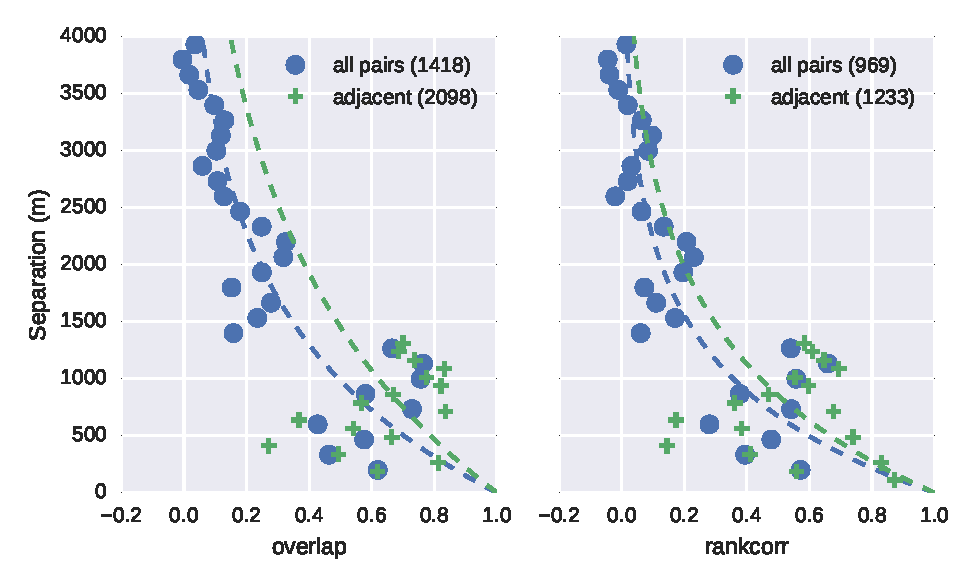
\includegraphics{graphics/subgrid2_overlap_dz.pdf}
\caption{\label{fig:subgrid2_overlap_dz}Global (area-weighted) average
cloud occurrence overlap parameter (left) and condensate rank
correlation (right) as a function of separation distance between layers
from a month of SP-CAM output. Also shown are fits to
eq.~\ref{eq:alpha_exponential_equation}, with values of decorrelation
length scales from these fits shown in the upper right corner of each
panel. Contours show the kernel density estimate for overlap and rank
correlation as a function of separation
distance.}\label{fig:subgrid2ux5foverlapux5fdz}
\end{figure}

Figure~\ref{fig:subgrid2_overlap_dz} shows the globally averaged overlap
and condensate rank correlation for total cloud condensate as a function
of separation distance (the area-weighted average of the overlap and
rank correlation calculated at each latitude-longitude gridbox). Overlap
and rank correlation are fit to eq.~\ref{eq:alpha_exponential_equation}
using non-linear least squares, and the fit is plotted on
Figure~\ref{fig:subgrid2_overlap_dz} as well, and the values of the
decorrelation lengths \(z_0\) from the fits are shown in each panel. The
globally averaged overlap and rank correlation statistics shown in
Figure~\ref{fig:subgrid2_overlap_dz} demonstrate the general tendency
for both overlap and rank correlation to decrease as the separation
between layers increases, and especially for distant layers the inverse
exponential dependence on separation distance following
eq.~\ref{eq:alpha_exponential_equation} seems reasonable. There is
however generally larger spread in cloud overlap and rank correlation
for small layer separations.

\begin{figure}[htbp]
\centering
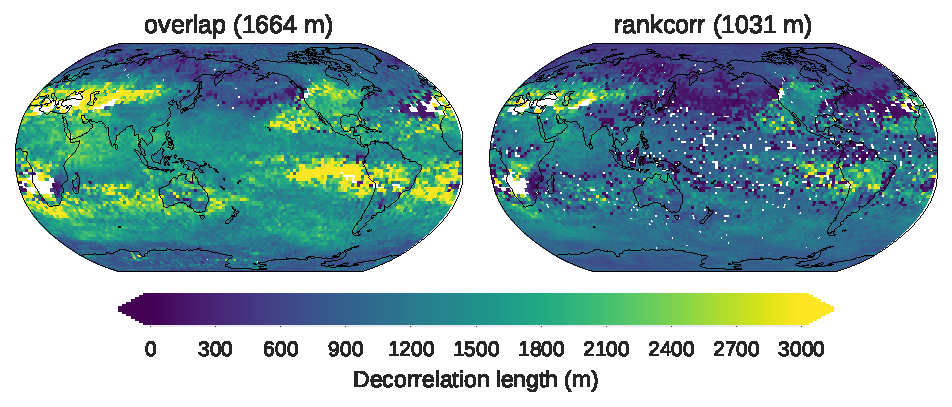
\includegraphics{graphics/subgrid2_overlap_maps.pdf}
\caption{\label{fig:subgrid2_overlap_maps}Maps of cloud occurrence
overlap (left) and condensate rank correlation (right) decorrelation
length scales for both cloud (top) and precipitation (bottom).
Decorrelation length scales at each point are calculated by fitting
time-averaged overlap and rank correlation as a function of separation
distance (in meters) to
eq.~\ref{eq:alpha_exponential_equation}.}\label{fig:subgrid2ux5foverlapux5fmaps}
\end{figure}

In order to derive decorrelation lengths for overlap and rank
correlation for use in the improved subcolumn generator presented here,
time-averaged overlap and rank correlation statistics are fit to
eq.~\ref{eq:alpha_exponential_equation} at each latitude-longitude
gridbox, and the decorrelation lengths from the fits are shown in
Figure~\ref{fig:subgrid2_overlap_maps} for overlap and rank correlation
binned by separation distance. This figure shows that both overlap and
rank correlation can vary substantially with geographic location, with
cloud overlap decorrelation lengths varying from less than 1 km to over
4 km. This suggests, as has been speculated by others \citep[
e.g.]{pincus_et_al_2005}, that overlap statistics are dependent on cloud
type. \citet{pincus_et_al_2005} speculated that overlap and rank
correlation are likely different for convective versus stratiform
clouds, with convective clouds likely more vertically coherent than
stratiform. The map shown in Figure~\ref{fig:subgrid2_overlap_maps} does
not seem entirely consistent with this assumption, however, as cloud
overlap and rank correlation decorrelation lengths are generally lower
throughout the deep tropics, and somewhat higher in the coastal
stratocumulus regions. The spatially varying patterns in decorrelation
lengths in Figure~\ref{fig:subgrid2_overlap_maps} suggest that assuming
a spatially invariant decorrelation length will likely lead to spatially
varying errors in cloud area. This is shown to be the case in the
following sections.

\begin{figure}[htbp]
\centering
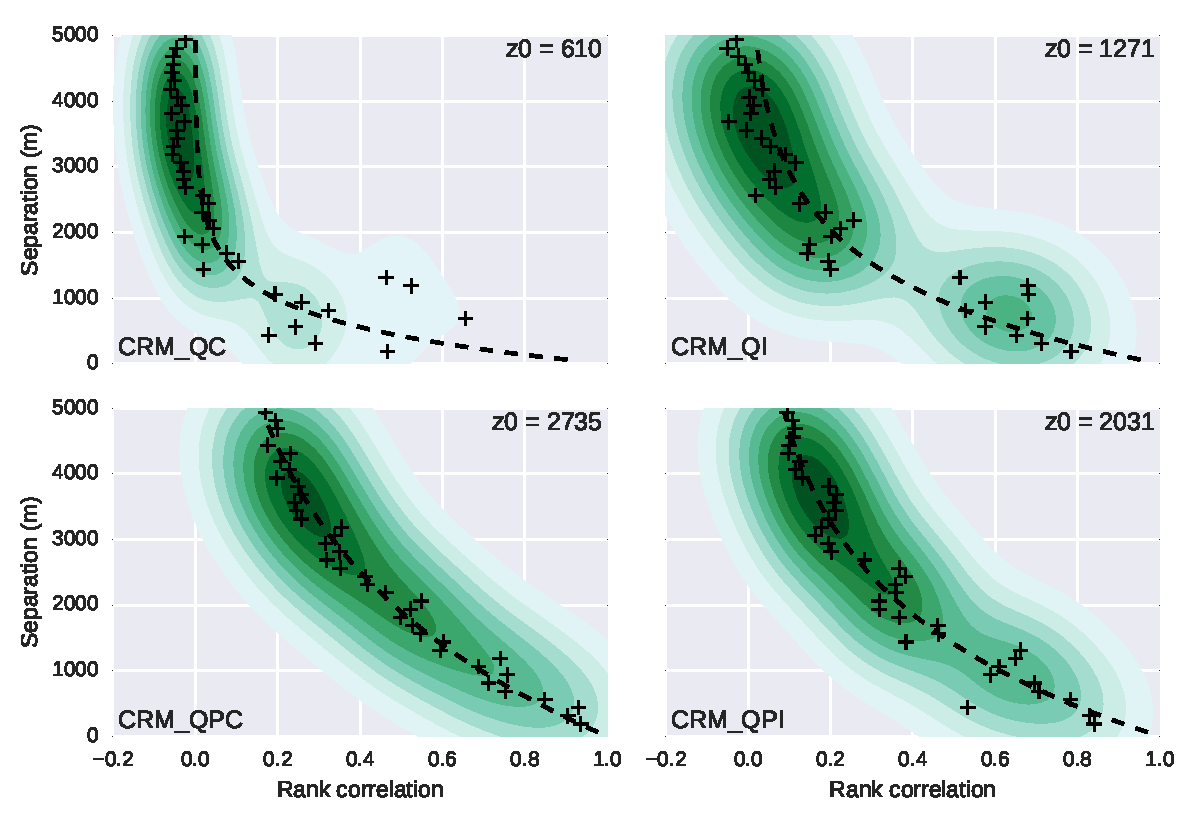
\includegraphics{graphics/subgrid2_rankcorr_dz.pdf}
\caption{\label{fig:subgrid2_rankcorr_dz}Time-averaged rank correlation
binned by separation distance for cloud liquid (CRM\_QC, upper left),
cloud ice (CRM\_QI, upper right), precipitating liquid (CRM\_QPC, lower
left), and precipitating ice (CRM\_QPI, lower right). Decorrelation
lengths fit to eq.~\ref{eq:alpha_exponential_equation} are shown in the
upper right of each panel.}\label{fig:subgrid2ux5frankcorrux5fdz}
\end{figure}

The subcolumn generator described in the previous sections allows for
generalized overlap of total cloud occurrence, using only the overlap
parameter between adjacent layers for total cloud. The method of
generating condensate distributions, however, in general allows for
separate rank correlations to be specified for each hydrometeor type
(cloud liquid, cloud ice, precipitating liquid, and precipitating ice).
Figure~\ref{fig:subgrid2_rankcorr_dz} shows global time-averaged rank
correlation as a function of separation distance, calculated as in
Figure~\ref{fig:subgrid2_overlap_dz} but for rank correlation instead of
occurrence overlap. The figure shows the clear dependence on separation
distance, with decreasing rank correlation with increasing separation,
but with decorrelation lengths varying widely between the different
hydrometeor types.

\begin{figure}[htbp]
\centering
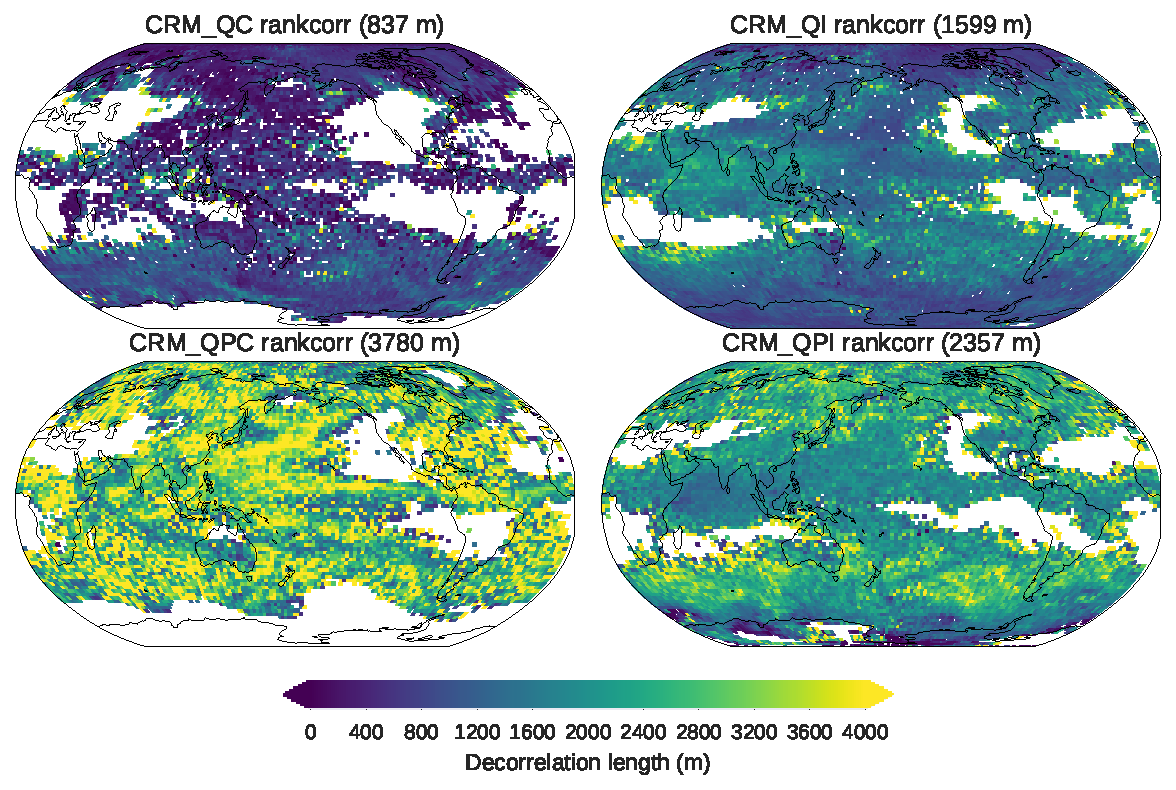
\includegraphics{graphics/subgrid2_rankcorr_maps.pdf}
\caption{\label{fig:subgrid2_rankcorr_maps}Decorrelation lengths for
condensate rank correlation for cloud liquid (CRM\_QC, upper left),
cloud ice (CRM\_QI, upper right), precipitating liquid (CRM\_QPC, lower
left), and precipitating ice (CRM\_QPI, lower
right).}\label{fig:subgrid2ux5frankcorrux5fmaps}
\end{figure}

The spatial dependence of the rank correlation is shown in
Figure~\ref{fig:subgrid2_rankcorr_maps}, which shows decorrelation
lengths fit separately for each gridbox as in
Figure~\ref{fig:subgrid2_overlap_maps} but for each hydrometeor type.
Rank correlation is seen to vary substantially with both hydrometeor
type and with location. Spatially coherent patterns similar to those for
cloud overlap are evident. Again, these results suggest that using
spatially invariant decorrelation lengths scales will predictably lead
to systematic biases in simulated diagnostics, but the point is to
evaluate the sensitivity to these assumptions relative to using the
maximum-random overlap assumption with horizontally homogeneous
condensate. Spatially invariant decorrelation length scales for
condensate rank correlation are taken from the cosine-latitude-weighted
global mean values, indicated above each panel in
Figure~\ref{fig:subgrid2_rankcorr_maps}.

\section{Parameterizing cloud and precipitation condensate
variability}\label{sec:subgrid2Variability}

To represent the subgrid-scale variability, it is assumed that the
subgrid-scale cloud and precipitation condensate mixing ratios (for
liquid and ice), each follow a gamma distribution, which has probability
density \[\begin{gathered}
p_{k, \theta}(q) = \frac{1}{\Gamma(k) \theta^k} q^{k - 1}
e^{-q/\theta}\end{gathered}\] where \(q\) is the condensate amount
(mixing ratio), \(k\) and \(\theta\) are the shape and scale parameters
of the gamma distribution, and \(\Gamma\) is the gamma function.
Previous authors have shown that condensate amounts can be fit well with
gamma, beta, or lognormal distributions \citep[e.g.;][]{lee_et_al_2010},
and it is shown here that gamma distributions are a reasonable fit to
the CRM fields produced by SP-CAM.
Figure~\ref{fig:subgrid2_condensate_cdf} shows the empirical cumulative
density function (CDF) for normalized cloud and precipitation condensate
\(q / \overline{q}\) for a single day of SP-CAM output, accumulated over
all columns and levels, along with fits to the gamma distribution. The
normalized condensate amount is used here because the global
distribution of condensate is dominated by the gridbox-mean condensate.
Scaling by the mean highlights the within-gridbox or subgrid-scale
variations, which is the type of heterogeniety that needs to be
parameterized for. The gamma CDF fits agree well with the empirical
CDFs, suggesting that the gamma distribution is consistent with
condensate distributions generated by the SP-CAM. {[}this needs a lot
more work/literature review{]}

\begin{figure}[htbp]
\centering
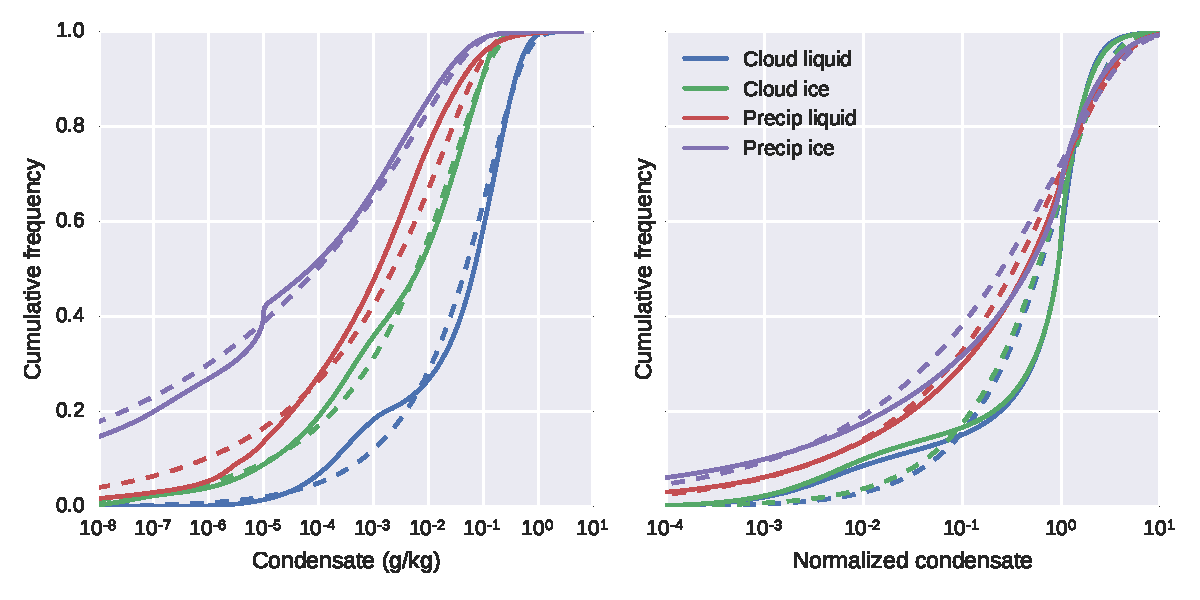
\includegraphics{graphics/subgrid2_mxratio_cdf1.pdf}
\caption{\label{fig:subgrid2_condensate_cdf}Raw (left) and normalized
(right) cloud and precipitation condensate mixing ratio empirical
cumulative density functions (solid curves), with fits to the gamma
distribution (dashed curves) for a single snapshot of SP-CAM
output.}\label{fig:subgrid2ux5fcondensateux5fcdf}
\end{figure}

The gamma distribution has mean \(\mu = k\theta\) and variance
\(\sigma^2 = k \theta^2\). Using the method of moments
\citep[e.g.;][]{wilks_2011} and equating the population mean and
variance with the sample mean \(\overline{q}\) and variance
\(\sigma_q^2\), this system of two equations is easily solved to
estimate the shape and scale parameters \(k = \mu^2 / \sigma_q^2\) and
\(\theta = \sigma_q^2 / \mu\). With this, the subgrid distribution of
condensate within each grid-box is completely specified in terms of the
grid-box mean and variance of condensate.

Cloud physics parameterizations in large-scale (global) models diagnose
the gridbox-mean cloud condensate amount, but most do not diagnose (or
even implicitly assume) the gridbox-variance. In order to build a simple
parameterization that could be used on typical GCM output, the
gridbox-variance in total cloud and total precipitation condensate
mixing ratio is represented here in terms of the gridbox-mean
condensate. Figure~\ref{fig:subgrid2_mxratio_variance} shows the
standard deviation in cloud liquid (upper left), cloud ice (upper
right), precipitating liquid (lower left) and precipitating ice (lower
right) condensate mixing ratios versus gridbox mean cloud and
precipitation condensate, respectively, again for a single snapshot of
SP-CAM output. Rather than show the scatter plot of the standard
deviation versus the mean, the figure shows a kernel density estimate
for the bivariate PDF of mean and standard deviation (shown by the
contours). Because the distribution of the mean and standard deviation
of condensate mixing ratios is strongly skewed, these are shown on a
log-log scale. The figure shows that the standard deviation of
condensate is strongly correlated with the mean, following an
approximately linear relationship in log-log space. This suggests that
the standard deviation \(\sigma\) can be represented in terms of the
mean \(\mu\) for each condensate type by the relationship
\(\sigma = a \mu^b\), where \(a\) and \(b\) are constants that need to
be parameterized. Note that taking the logarithm of both sides shows
that this leads to a linear relationship in log-log space:
\[\begin{gathered}
\log \sigma = \log(a \mu^b) = \log a + b\log \mu\end{gathered}\]
Standard deviation is then fit to \(\sigma = a \mu^b\) by performing a
linear regression of \(\log\sigma\) versus \(\log \mu\) to estimate the
slope and intercept \(a^{\prime}\) and \(b^{\prime}\) in
\(\log \sigma = a^{\prime} \log \mu + b^{\prime}\), and then determining
\(a\) and \(b\) such that \(\sigma = a \mu^b\) by taking
\(a = 10^{b^{\prime}}\) and \(b = a^{\prime}\). That is, the fit is
performed in log-log space, and the fit parameters are then transformed
back. The fit parameters \(a\) and \(b\), as well as the coefficient of
determination \(r^2\) (from the linear regression in log-log space) are
indicated in each panel of Figure~\ref{fig:subgrid2_mxratio_variance}
for the example SP-CAM snapshot. This fit is repeated for each 3-hourly
snapshot of SP-CAM output in the month of July 2000 (248 total
snapshots), and the fit parameters for each snapshot are shown in
Figure~\ref{fig:subgrid2_mxratio_variance_fits}. The fit parameters are
then averaged over all of the snapshots to provide a single
parameterization of the scale and power parameters \(a\) and \(b\) for
use in the sensitivity tests in this chapter. The averages of the fit
parameters are shown in Table
Table~\ref{tbl:subgrid2_mxratio_variance_fits_table}

\begin{figure}[htbp]
\centering
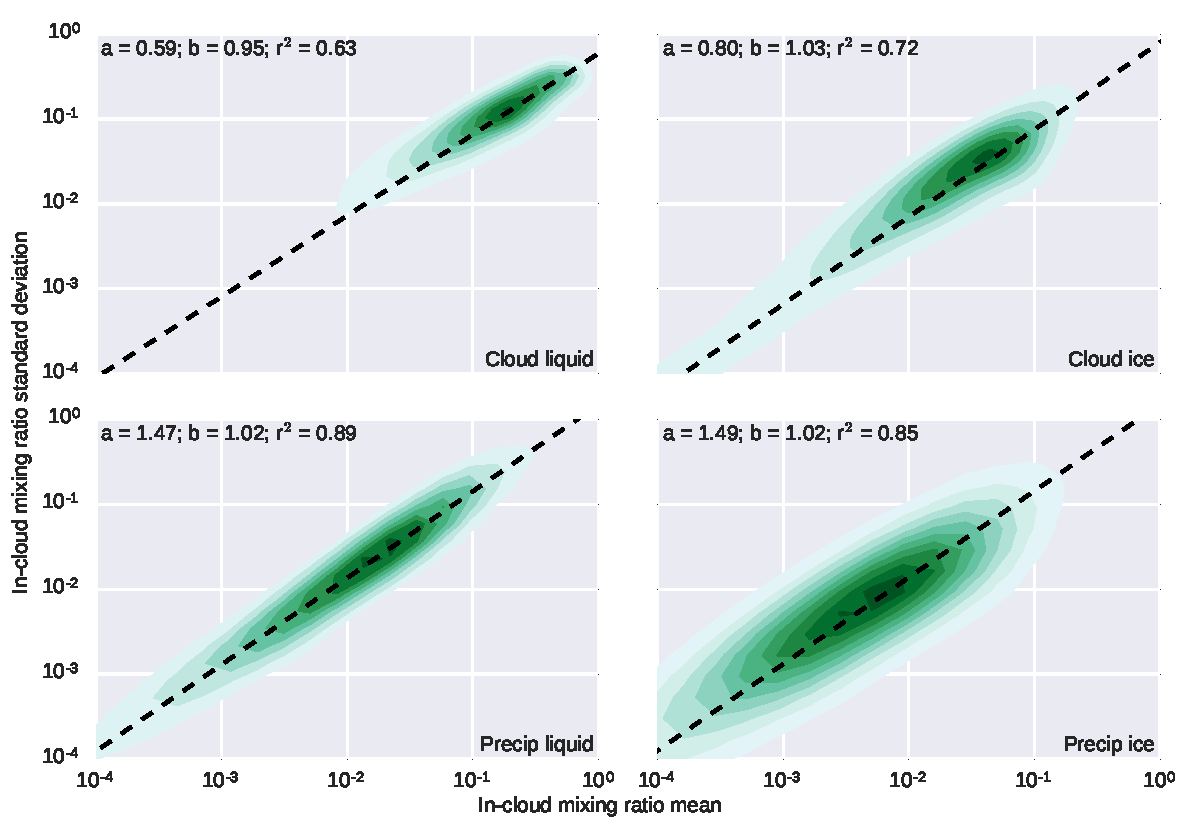
\includegraphics{graphics/subgrid2_mxratio_variance.pdf}
\caption{\label{fig:subgrid2_mxratio_variance}Kernel density estimate
for the bivariate PDF of condensate standard deviation and mean for
cloud liquid, cloud ice, precipitating liquid, and precipitating ice
(contours) for a single global snapshot of SP-CAM CRM output. Shown in
the upper left corner of each panel are the fit parameters to the
relationship \(\sigma = a \mu^b\), along with the coefficient of
determination (\(r^2\)) of the
fit.}\label{fig:subgrid2ux5fmxratioux5fvariance}
\end{figure}

\begin{figure}[htbp]
\centering
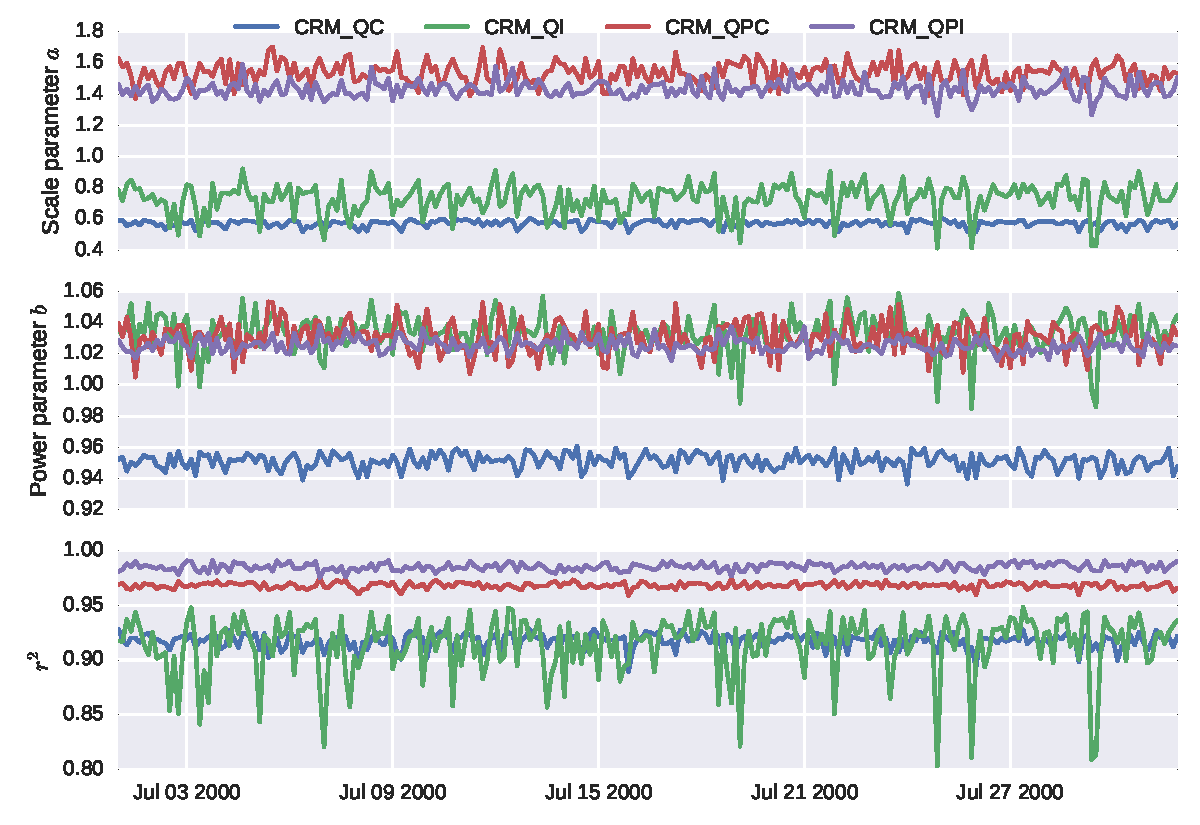
\includegraphics{graphics/subgrid2_mxratio_variance_fits.pdf}
\caption{\label{fig:subgrid2_mxratio_variance_fits}Fits to
\(\sigma = a \mu^b\) for each of the 248 SP-CAM snapshots in July
2000.}\label{fig:subgrid2ux5fmxratioux5fvarianceux5ffits}
\end{figure}

\begin{longtable}[]{@{}lccc@{}}
\caption{\label{tbl:subgrid2_mxratio_variance_fits_table}Averages of the
fit parameters shown in Figure~\ref{fig:subgrid2_mxratio_variance_fits}
over all 284 SP-CAM snapshots. }\tabularnewline
\toprule
& Average \(a\) & Average \(b\) & Average \(r^2\)\tabularnewline
\midrule
\endfirsthead
\toprule
& Average \(a\) & Average \(b\) & Average \(r^2\)\tabularnewline
\midrule
\endhead
Cloud liquid & 0.57 & 0.95 & 0.92\tabularnewline
Cloud ice & 0.73 & 1.03 & 0.91\tabularnewline
Precip liquid & 1.54 & 1.03 & 0.97\tabularnewline
Precip ice & 1.43 & 1.03 & 0.99\tabularnewline
\bottomrule
\end{longtable}

This provides a simple parameterization for condensate standard
deviation, so that given just the gridbox mean values at each level,
condensate standard deviation can be represented using this functional
relationship. To generate stochastic subcolumns of clouds and
precipitation using this, subcolumn cloud and precipitation occurrence
flags are first generated using the framework described in
Section~\ref{sec:subgrid2Generator}. Condensate amount is then generated
for each hydrometeor type (cloud liquid, cloud ice, precipitating
liquid, precipitating ice) using the framework described there, assuming
that each hydrometeor type occupies all of the cloudy or precipitating
subcolumn elements, using the above parameterization to specify the
standard deviation in terms of the mean.

As discussed in the previous section in the context of the
parameterization of overlap and rank correlation, these relationships
are unlikely to hold under all conditions and cloud regimes, but this
simple parameterization is sufficient for testing the sensitivity of
simulated satellite cloud diagnostics to the treatment of unresolved
variability. With overlap, rank correlation, and condensate
distributions completely parameterized, an additional set of modified
fields is created using the above described subcolumn generator, and
referred to as ``GEN-VAR-PARAM''. In order to separately test the
parameterization of overlap, rank correlation, and variability, another
set of modified fields is created where the overlap, rank correlation,
and gridbox variance is calculated at each gridbox directly from the CRM
fields rather than parameterized. This case is referred to as
``GEN-VAR-CALC'' and represents the limit of performance that can be
expected with this subcolumn generator.

\begin{figure}[htbp]
\centering
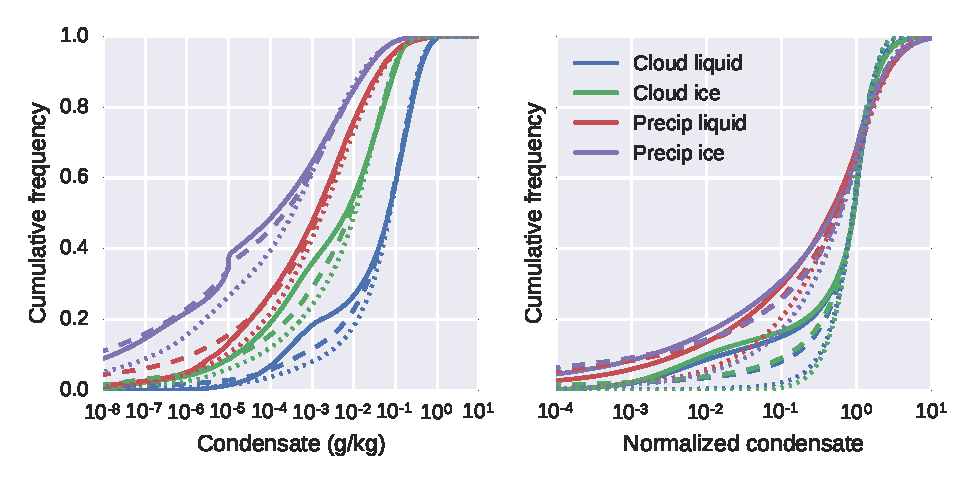
\includegraphics{graphics/subgrid2_mxratio_cdf2.pdf}
\caption{\label{fig:subgrid2_condensate_cdf2}Raw (left) and normalized
(right) condensate empirical density functions from the CRM,
GEN-VAR-PARAM, and GEN-VAR-CALC cases as described in the text for a
single snapshot of SP-CAM
output.}\label{fig:subgrid2ux5fcondensateux5fcdf2}
\end{figure}

Figure~\ref{fig:subgrid2_condensate_cdf2} shows the cumulative
distributions of condensate amounts for each hydrometeor type from the
regenerated GEN-VAR-PARAM (dotted curves) and GEN-VAR-CALC (dashed
curves) cases for a single snapshot of SP-CAM output, as compared with
the CDFs from the original CRM fields (solid curves) as shown in
Figure~\ref{fig:subgrid2_condensate_cdf}. The figure shows that the
GEN-VAR-CALC case is able to reasonably reproduce the distribution of
both the raw condensate and of the normalized condensate for each
hydrometeor type. The distributions from the GEN-VAR-PARAM case (using
the parameterization for variance described above) seem to reproduce the
raw condensate reasonably well, but do not do as well at reproducing the
distribution of normalized condensate for any hydrometeor type. In
general the parameterization tends to underestimate the number of
hydrometeors with very small values relative to the mean, with larger
values of condensate mixing ratios making up the majority of the
distribution. It is clear that the parameterization leaves a lot of room
for improvement, but it is stressed that the purpose here is not to
develop a perfect parameterization that can be immediately implemented
into a large-scale model, but rather to demonstrate the sensitivity of
satellite-simulated diagnostics from COSP to improvements in the
treatment of variability and overlap. The simple parameterization
presented here is sufficient to accomplish this.

The sensitivity test framework uses outputs from the SP-CAM to provide a
plausible representation of cloud and precipitation structure and
variability at scales similar to those at which the satellite retrievals
are performed. While these outputs provide much higher resolution cloud
fields than available in traditional GCMs, the fields simulated by the
SP-CAM are in fact still model outputs, and may not perfectly simulate
any observed cloud systems. Nonetheless, it has been shown here that the
overlap and rank correlation statistics from SP-CAM are both
qualitatively and quantitatively consistent with those found in
observations from previous authors, and condensate variability is at
least qualitatively consistent with previous studies as well, following
similar statistical distributions. Thus, since the goal of this study is
to evaluate the sensitivity of COSP diagnostics to these properties,
rather than to develop a perfect parameterization of subgrid-scale
overlap and variability, the SP-CAM output is sufficient for this
purpose. In order to run the individual simulators directly on output
from the SP-CAM, it is important that the fields simulated by the SP-CAM
are on a scale similar to that at which the satellite retrievals are
performed. The SP-CAM output used in this study was run using 4 km grid
spacing for the embedded cloud-resolving model. MISR cloud top height
retrievals are performed at a spatial scale of 1.1 km
\citep{moroney_et_al_2002}, and the CloudSat cloud radar has a
horizontal resolution of 1.4 km cross-track and 1.7 km along-track
\citep{tanelli_et_al_2008}. While these scales are somewhat smaller than
the 4 km grid used by the SP-CAM CRM, the differences are small and are
unlikely to affect the results of the sensitivity study performed with
the 4 km fields.

\section{Quantifying improvements in COSP-simulated
diagnostics}\label{sec:subgrid2Results}

With the improved subcolumn generator described in the preceeding
sections, the sensitivity of the COSP diagnostics to the improvements
can be quantified using the same framework used in the previous chapter
to quantify the sensitivities to overlap and homogeneous condensate
assumptions. Again, a series of modified cloud and precipitation
condensate fields are created from a month-long SP-CAM simulation. COSP
is then run on each set of modified fields, and the COSP outputs are
compared with one another to quantify the sensitivity to different
aspects of the improved subcolumn generator. These cases are described
below.

\begin{figure}[htbp]
\centering
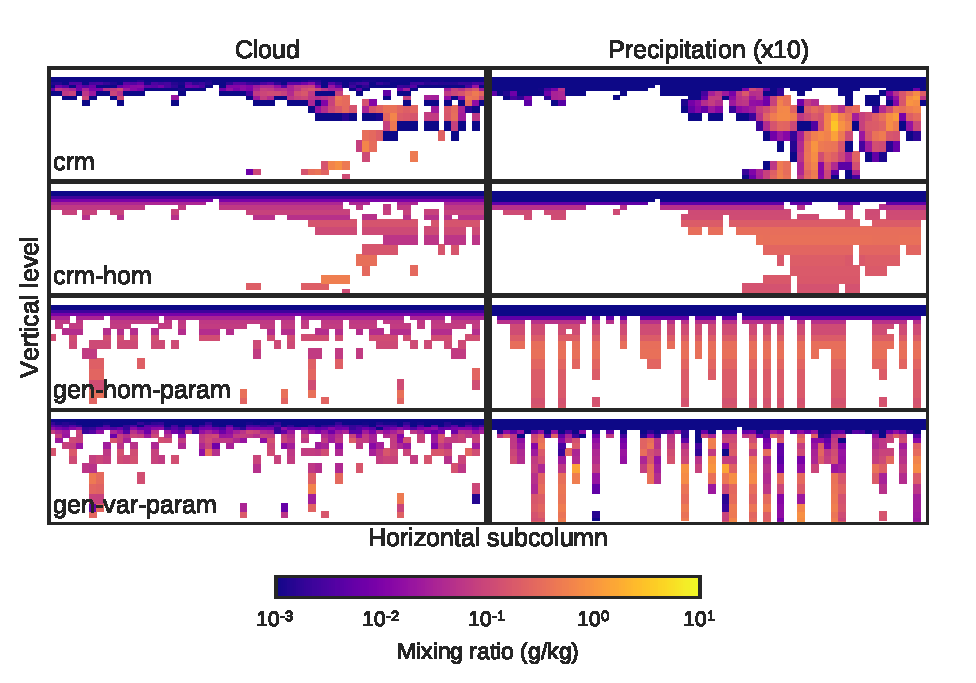
\includegraphics{graphics/subgrid2_mxratio_example.pdf}
\caption{\label{fig:subgrid2_mxratio_example}Cases with improved
subcolumn generator following
R04.}\label{fig:subgrid2ux5fmxratioux5fexample}
\end{figure}

The first two cases are identical to those used in the previous chapter.
The first is the baseline (CRM) case, created by running COSP on the
original, unmodified CRM fields from the SP-CAM simulation. The second
case is the homogenized case (CRM-HOM), created by replacing the cloud
and precipitation condensate with the gridbox-means (by level),
everywhere where cloud and precipitation exist in the original CRM
fields. The remaining cases are generated as in
Section~\ref{sec:subgrid1} by first calculating the gridbox-mean
profiles of cloud fraction, precipitation fraction, and cloud and
precipitation condensate (for each hydrometeor type) from the original
CRM fields, and then using the new subcolumn generator to regenerate
subcolumn condensate fields from the gridbox-mean profiles. Four such
cases are created using the new subcolumn generator: two with calculated
overlap and variance, and two with parameterized overlap and variance.

The first of these uses the new subcolumn generator described above with
generalized overlap and horizontally variable condensate, but with
overlap, rank correlation, and variance calculated directly from the
original CRM fields at each gridbox and time step rather than
parameterized (GEN-VAR-CALC). Because this case uses the R04 scheme but
with overlap, rank correlation, and variance calculated from the
original fields rather than parameterized, this case represents the
limit of the performance that can be expected from this subcolumn
scheme, if these parameters could be perfectly prescribed. The second
regenerated case uses only the generalized cloud overlap part of the R04
scheme, combined with horizontally homogeneous cloud and precipitation
condensate (in the same manner as the MRO-HOM-PADJ case in
Section~\ref{sec:subgrid1}). This case will be used to separate out
errors due to the treatment of overlap and due to the treatment of
variability in the same manner as in Section~\ref{sec:subgrid1}, and as
described below.

The third regenerated case uses the full subcolumn generator with
overlap, rank correlation, and variance parameterized as described above
(GEN-VAR-PARAM). The parameterization of these quantities was seen in
the previous section to be less than ideal, so it is not expected that
this case will perfectly reproduce the characteristics of the original
CRM case. Rather, this case represents the performance that can be
expected from the R04 generator with a simple parameterization of
overlap, rank correlation, and condensate gridbox-variance. A fourth
case is created that again uses only the generalized cloud overlap
treatment part of the R04 scheme to separate out the errors due to
overlap and due to the treatment of variability, as described in the
following paragraph.

As in the previous chapter, the sensitivity to both the overlap and the
variability treatment can be quantified by taking appropriate
differences between the outputs from these different cases. The CRM-HOM
and GEN-HOM-PARAM (and GEN-HOM-CALC) cases differ primarily in the
treatment of cloud (and precipitation) overlap, so the difference
between the outputs from these cases quantifies the component of the
error due to the generalized overlap treatment alone. This will be
calculated for both the GEN-HOM-CALC case and for the GEN-HOM-PARAM
case, showing both the generalized overlap errors that can be achieved
with ideal overlap and with overlap specified only by a monthly and
spatially invariant (averaged) decorrelation length. The component of
the error due to the treatment of variability is quantified by
calculating the residual between the total error in using the full
subcolumn generator (GEN-VAR-CALC or GEN-VAR-PARAM minus CRM) and the
component of the error due to the treatment of overlap (GEN-HOM-CALC or
GEN-HOM-PARAM minus CRM-HOM). The total error \(E_\textrm{total}\) and
the overlap and variability components \(E_\textrm{overlap}\) and
\(E_\textrm{variability}\) are calculated for a simulated satellite
diagnostic quantity \(X\) then as \[\begin{gathered} E_\textrm{total} =
X_\textrm{GEN-VAR} - X_\textrm{CRM} \\ E_\textrm{overlap} = X_\textrm{GEN-HOM} -
X_\textrm{CRM-HOM} \\ E_\textrm{variability} = (X_\textrm{GEN-VAR} -
X_\textrm{CRM}) - (X_\textrm{GEN-HOM} - X_\textrm{CRM-HOM})\end{gathered}\]
The sensitivity of the various simulated diagnostics to the
modifications made in the new subcolumn generator are evaluated using
this framework in the following sections.

\section{Reduced errors in simulated passive remote sensing
diagnostics}\label{sec:subgrid2Passive}

\begin{figure}[htbp]
\centering
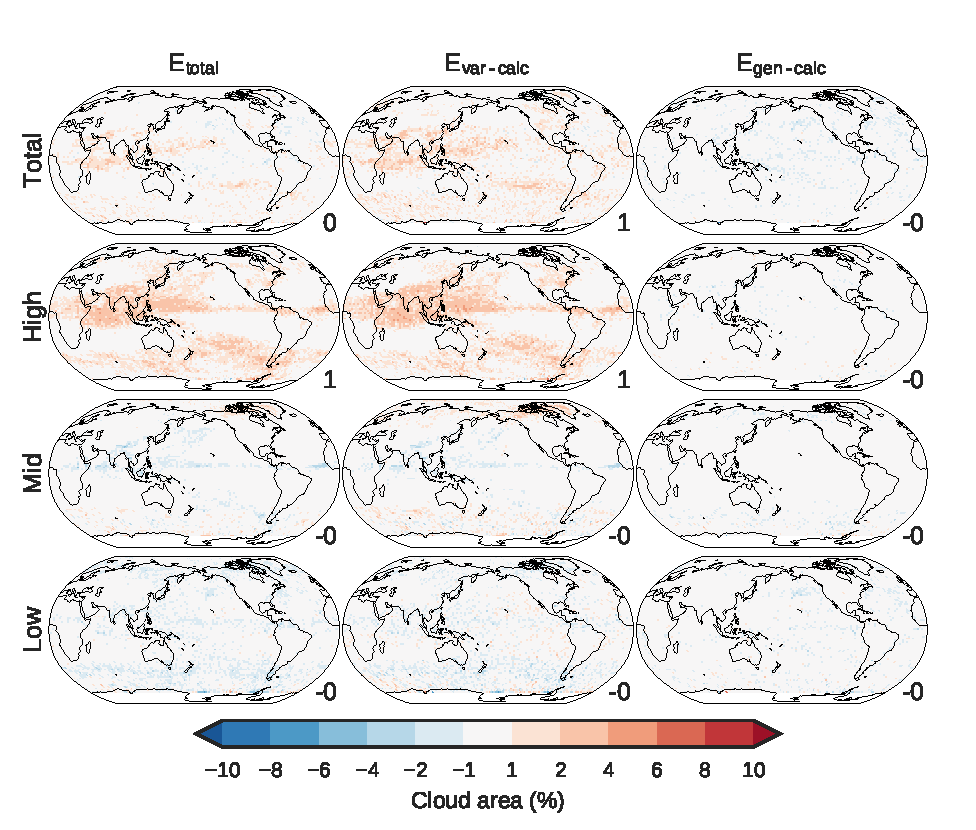
\includegraphics{graphics/subgrid2_cldmisr_maps_gen-var-calc_diff.pdf}
\caption{\label{fig:subgrid2_cldmisr_maps_gen-var-calc_diff}Errors in
MISR-simulated cloud area by cloud top height arising due to using the
improved GEN-VAR subcolumn generator with \emph{calculated} overlap and
variability to regenerate subcolumns from gridbox-mean profiles (left),
the component of the error due to the treatment of variability (middle),
and the component of the error due to the treatment of overlap
(right).}\label{fig:subgrid2ux5fcldmisrux5fmapsux5fgen-var-calcux5fdiff}
\end{figure}

\begin{figure}[htbp]
\centering
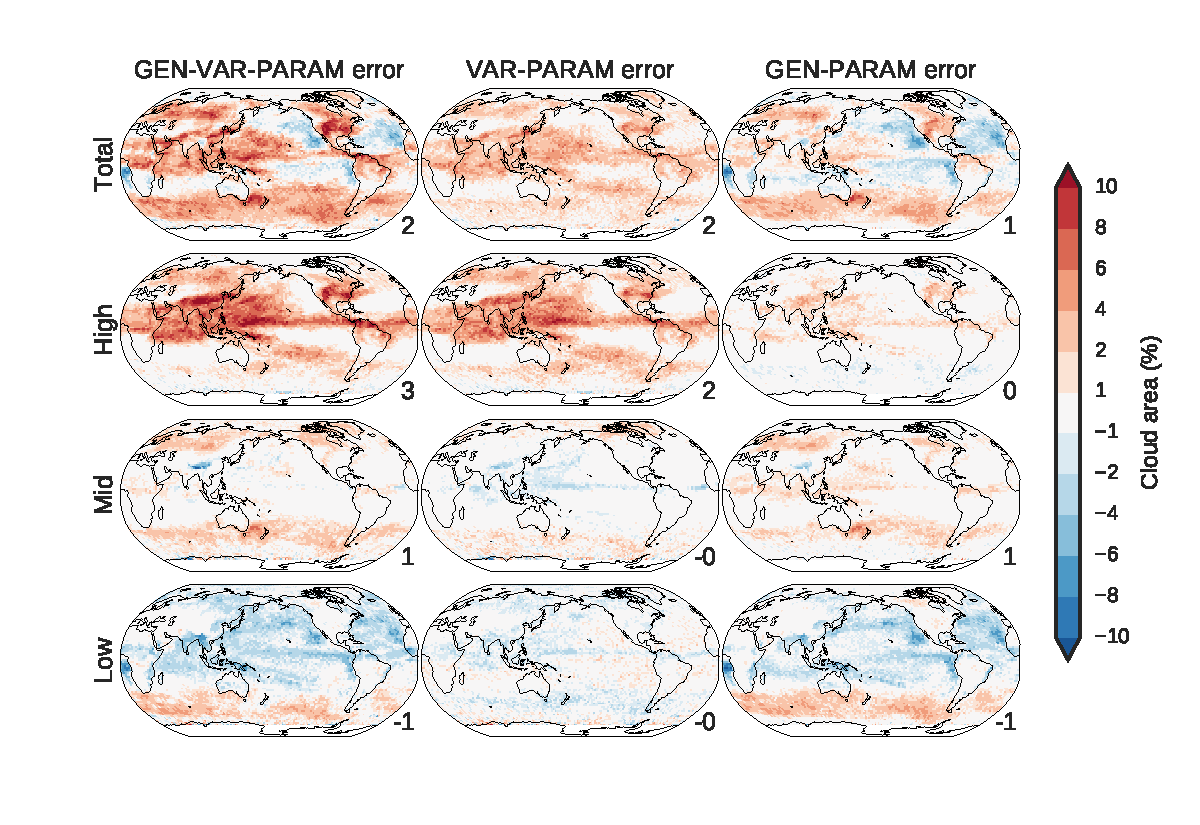
\includegraphics{graphics/subgrid2_cldmisr_maps_gen-var-param_diff.pdf}
\caption{\label{fig:subgrid2_cldmisr_maps_gen-var-param_diff}Errors in
MISR-simulated cloud area by cloud top height arising due to using the
improved GEN-VAR subcolumn generator with \emph{parameterized} overlap
and variability to regenerate subcolumns from gridbox-mean profiles
(left), the component of the error due to the treatment of variability
(middle), and the component of the error due to the treatment of overlap
(right).}\label{fig:subgrid2ux5fcldmisrux5fmapsux5fgen-var-paramux5fdiff}
\end{figure}

Figure~\ref{fig:subgrid2_cldmisr_maps_gen-var-calc_diff} and
Figure~\ref{fig:subgrid2_cldmisr_maps_gen-var-param_diff} show the
errors in MISR-simulated cloud area by cloud top height that arise due
to using the new GEN-VAR subcolumn generator to regenerate subcolumn
cloud and precipitation condensate fields from gridbox-mean profiles, in
the same manner in which Figure~\ref{fig:subgrid1_cldmisr_maps_diff}
shows errors that arise due to using SCOPS/PREC\_SCOPS with
maximum-random overlap and homogeneous condensate (MRO-HOM).
Figure~\ref{fig:subgrid2_cldmisr_maps_gen-var-calc_diff} shows the
errors in using the new scheme with ideal or ``best-case'' overlap, rank
correlation, and variance calculated directly from the original CRM
fields, while Figure~\ref{fig:subgrid2_cldmisr_maps_gen-var-param_diff}
shows the errors in using the new scheme with these quantities
parameterized as discussed in
Sections~\ref{sec:subgrid2Overlap}, \ref{sec:subgrid2Variability}.
Comparing Figure~\ref{fig:subgrid2_cldmisr_maps_gen-var-calc_diff} and
Figure~\ref{fig:subgrid1_cldmisr_maps_diff} it is clear that the GEN-VAR
scheme with ideal overlap and variability is able to substantially
reduce the errors identified in Section~\ref{sec:subgrid1} due to both
the treatment of variability and overlap. Errors due to the treatment of
variability are everywhere less than 6\% (and generally much smaller,
between 0 and 2\%) cloud area using the new scheme, compared with errors
as large as 10\% cloud area using homogeneous condensate. Errors due to
the overlap treatment are similarly reduced, from regional errors as
large as 10\% using MRO down to less than 2\% using the GEN-VAR scheme.
The total error that arises due to regenerating subcolumns using the
subcolumn generator has likewise been reduced, but more importantly the
compensating errors between high and low-topped clouds have been nearly
eliminated using the new scheme.

Using parameterized overlap, rank correlation, and variance results in
larger errors than using the calculated values, as seen in
Figure~\ref{fig:subgrid2_cldmisr_maps_gen-var-param_diff}. The errors
due to the treatment of variability are comparable to those that result
from using homogeneous condensate, seen in
Figure~\ref{fig:subgrid1_cldmisr_maps_diff}. High-topped cloud
especially is overestimated throughout the tropical western pacific.
Errors due to using parameterized overlap show clear spatial patterns,
with overestimation of cloud area especially in the southern ocean but
also somewhat in the tropical western pacific and over the continents,
and an underestimation of cloud area elsewhere. The majority of these
errors (especially in the southern ocean) appear to be in the low-topped
cloud area. These errors, especially in the southern ocean low-topped
cloud, have a similar spatial structure to the global map of
decorrelation length shown in Figure~\ref{fig:subgrid2_overlap_maps}.
The errors due to using the parameterized overlap suggest that using a
globally constant decorrelation length for cloud occurrence overlap is
insufficient to characterize the overlap of clouds simulated by SP-CAM
(and likely real clouds in the physical atmosphere). Nonetheless, the
results of Figure~\ref{fig:subgrid2_cldmisr_maps_gen-var-calc_diff}
demonstrate the promise of using the improved subcolumn generator with
COSP, and suggest that future research to improve the characterization
of overlap statistics and horizontal variability in large-scale models
would be a worthwhile endeavor.

\section{Reduced errors in simulated CloudSat reflectivity and
hydrometeor occurrence}\label{sec:subgrid2Active}

\begin{figure}[htbp]
\centering
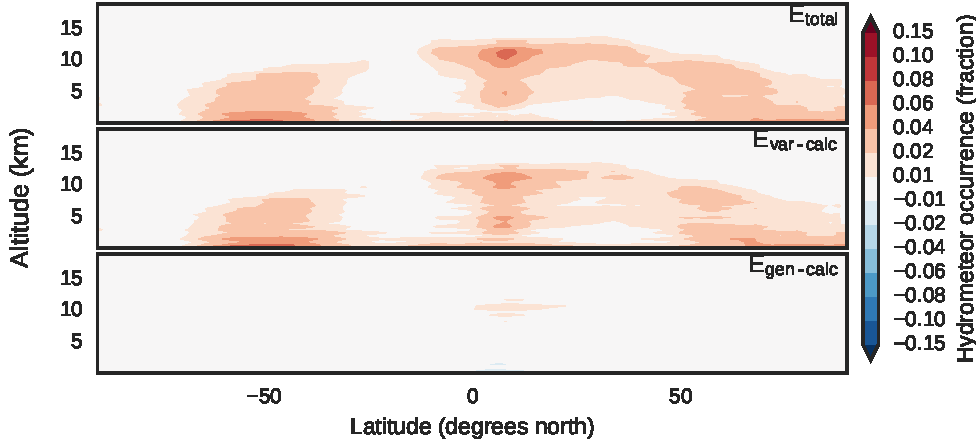
\includegraphics{graphics/subgrid2_hfba_zonal_gen-var-calc_diff.pdf}
\caption{\label{fig:subgrid2_hfba_zonal_diff}Errors in
CloudSat-simulated hydrometeor occurrence (\(Z_e > -27.5\) dBZ) arising
due to using GEN-VAR with calculated overlap and variability to
regenerate subcolumns of cloud and precipitation (top), as well as
components due to both the VAR treatment of variability (middle) and the
GEN treatment of overlap
(bottom).}\label{fig:subgrid2ux5fhfbaux5fzonalux5fdiff}
\end{figure}

\begin{figure}[htbp]
\centering
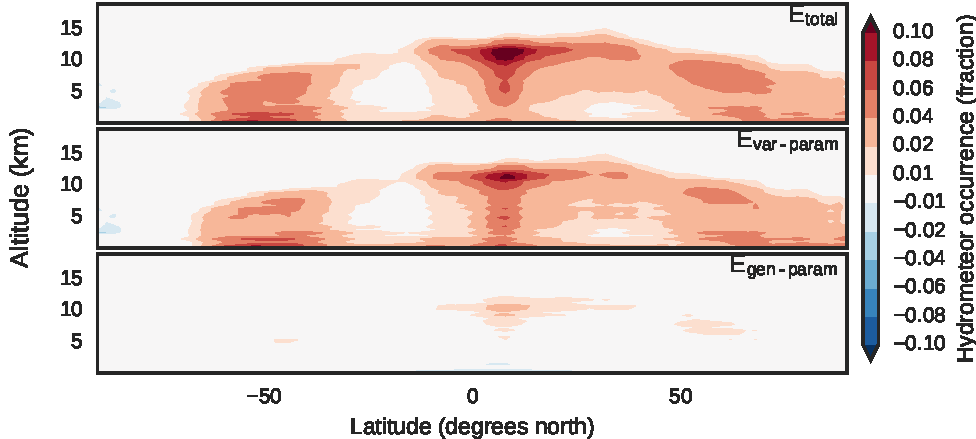
\includegraphics{graphics/subgrid2_hfba_zonal_gen-var-param_diff.pdf}
\caption{\label{fig:subgrid2_hfba_zonal_gen-var-param_diff}Errors in
CloudSat-simulated hydrometeor occurrence (\(Z_e > -27.5\) dBZ) arising
due to using GEN-VAR with parameterized overlap and variability to
regenerate subcolumns of cloud and precipitation (top), as well as
components due to both the VAR treatment of variability (middle) and the
GEN treatment of overlap
(bottom).}\label{fig:subgrid2ux5fhfbaux5fzonalux5fgen-var-paramux5fdiff}
\end{figure}

Figure~\ref{fig:subgrid2_hfba_zonal_diff} and
Figure~\ref{fig:subgrid2_hfba_zonal_gen-var-param_diff} show the errors
in the zonally-averaged CloudSat-simulated hydrometeor occurrence
fraction. Comparing these errors to those shown in
Figure~\ref{fig:subgrid1_hfba_zonal_diff} again shows a substantial
reduction in errors of all types using the improved subcolumn generator
relative to those errors that resulted from using SCOPS/PREC\_SCOPS when
using the ideal (calculated) overlap and variance. The total error that
arises using the GEN-VAR-CALC scheme to regenerate subcolumns results in
errors that are generally less than 0.06 frequency of occurrence,
compared to errors will above 0.1 frequency of occurrence using the old
SCOPS/PREC\_SCOPS routine. The remaining errors appear to be almost
entirely due to the treatment of variability, and the component of the
error due to the treatment of cloud overlap is nearly zero. {[}Need to
comment on why variability errors remain non-zero; I think due to
cross-correlation of cloud and precipitation occurrence and condensate
amount{]}

Errors in CloudSat-simulated hydrometeor occurrence when using the
parameterized treatment of overlap and variability are much larger than
when using the calculated overlap and variability. While the errors due
to the treatment of overlap remain small, the errors due to the
treatment of variability are substantially larger. Still, these errors
are generally less than arise when using homogeneous cloud and
precipitation condensate (compare with
Figure~\ref{fig:subgrid1_hfba_zonal_diff}), indicating that even the
simple parameterization of variability used here is an improvement over
the original subgrid generator with horizontally homogeneous condensate.

\begin{figure}[htbp]
\centering
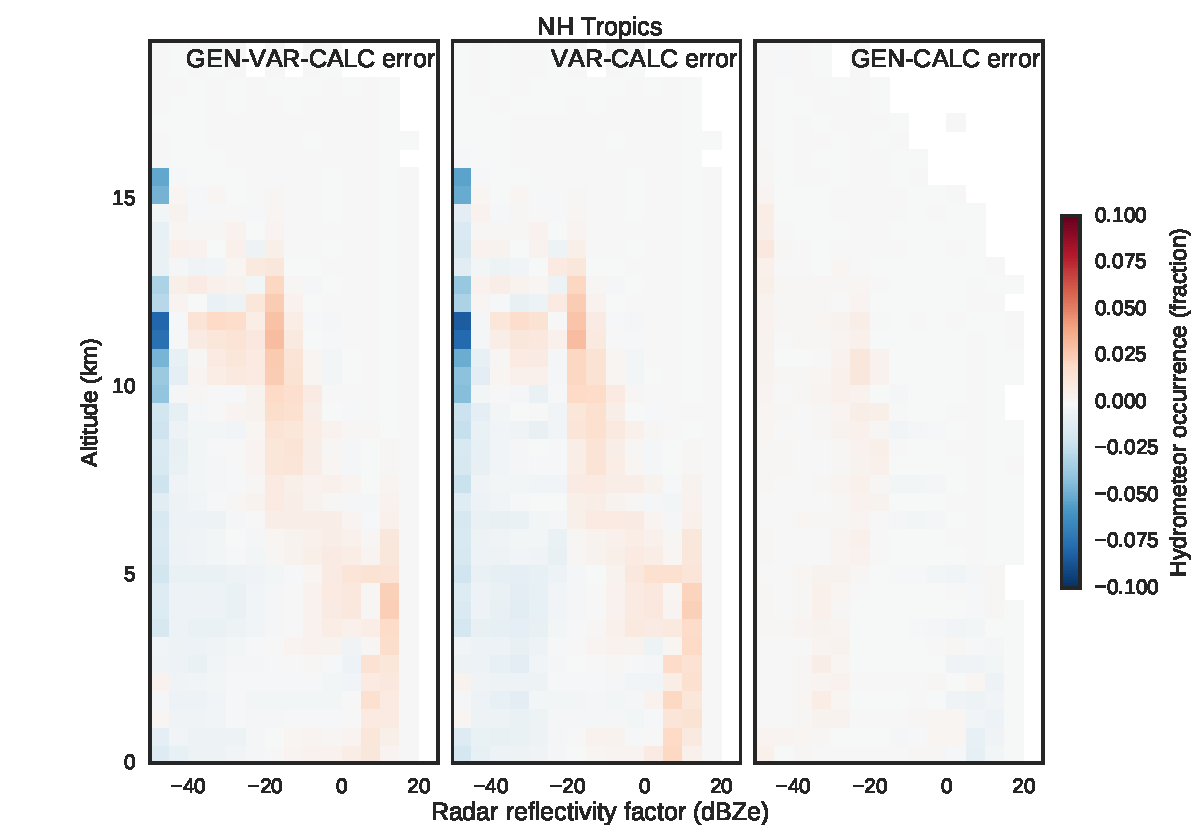
\includegraphics{graphics/subgrid2_cfadDbze94_NHTropics_gen-var-calc_diff.pdf}
\caption{\label{fig:subgrid2_cfadDbze94_nhtropics_diff}Errors in
CloudSat-simulated reflectivity with height histograms for the NH
Tropics (0 to 10 degrees
north).}\label{fig:subgrid2ux5fcfadDbze94ux5fnhtropicsux5fdiff}
\end{figure}

\begin{figure}[htbp]
\centering
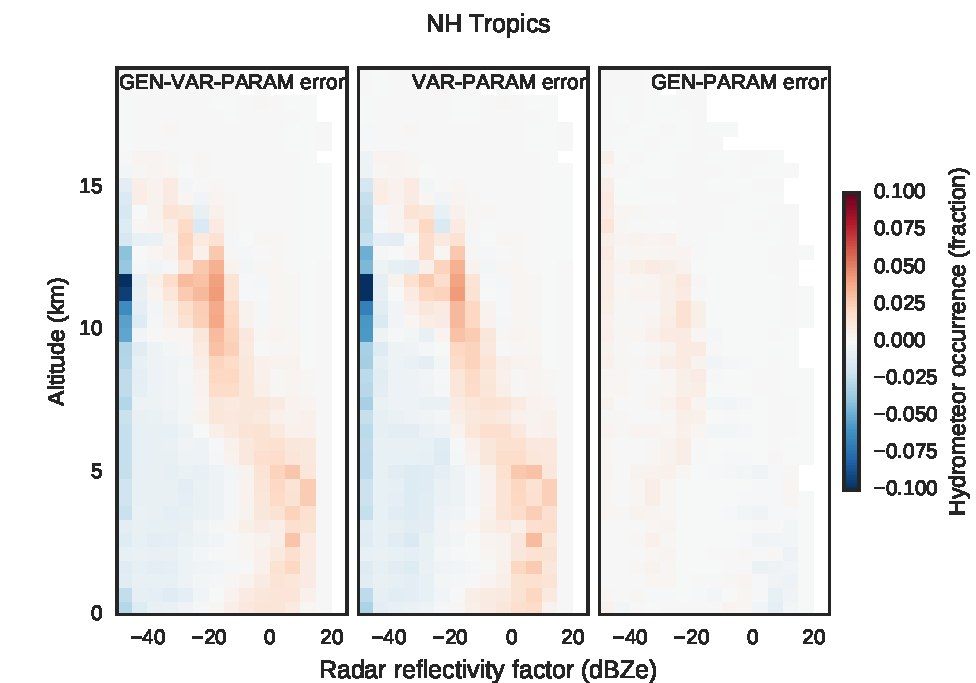
\includegraphics{graphics/subgrid2_cfadDbze94_NHTropics_gen-var-param_diff.pdf}
\caption{\label{fig:subgrid2_cfadDbze94_nhtropics_gen-var-param_diff}Errors
in CloudSat-simulated reflectivity with height histograms for the NH
Tropics (0 to 10 degrees
north).}\label{fig:subgrid2ux5fcfadDbze94ux5fnhtropicsux5fgen-var-paramux5fdiff}
\end{figure}

Figure~\ref{fig:subgrid2_cfadDbze94_nhtropics_diff} and
Figure~\ref{fig:subgrid2_cfadDbze94_nhtropics_gen-var-param_diff} show
errors in CloudSat-simulated reflectivity with height histograms for the
Northern Hemisphere Tropics. The figures show again a reduction in
errors of all types from using the new subcolumn scheme with either
calculated or parameterized overlap and variability to regenerate
subcolumns compared with the errors identified in
Figure~\ref{fig:subgrid1_cfadDbze94_tropics_diff}. The largest impact is
the inclusion of heterogeneous condensate, as after adjusting for
precipitation, the homogeneous errors dominated the errors using MRO-HOM
scheme shown in the previous chapter. Again, errors are somewhat larger
using the parameterized variance treatment, while the error due to using
the parameterized overlap treatment remains small. Similar to the
homogeneous errors identified in Section~\ref{sec:subgrid1} (
Figure~\ref{fig:subgrid1_cfadDbze94_tropics_diff}), errors due to the
parameterized variance manifest in a decrease in occurrence of
low-reflectivity hydrometeors and an increase in occurrence of
hydrometeors with higher reflectivity along the characteristic curve of
reflectivity with height. Still, these errors are substantially smaller
than arise when using homogeneous condensate.
Figure~\ref{fig:subgrid2_cfadDbze94_NHTropics_all_diff} shows the total
errors from using each configuration of subcolumn generators, including
SCOPS/PREC\_SCOPS, SCOPS/PREC\_SCOPS with the precipitation adjustment,
the new subcolumn generator with calculated overlap and variance, and
the new subcolumn generator with parameterized overlap and variance. It
is obvious that although the errors using parameterized overlap and
variance are larger than when using calculated overlap and variance,
these errors are much smaller than when using SCOPS/PREC\_SCOPS with
homogeneous condensate, especially at lower-altitudes.

\begin{figure}[htbp]
\centering
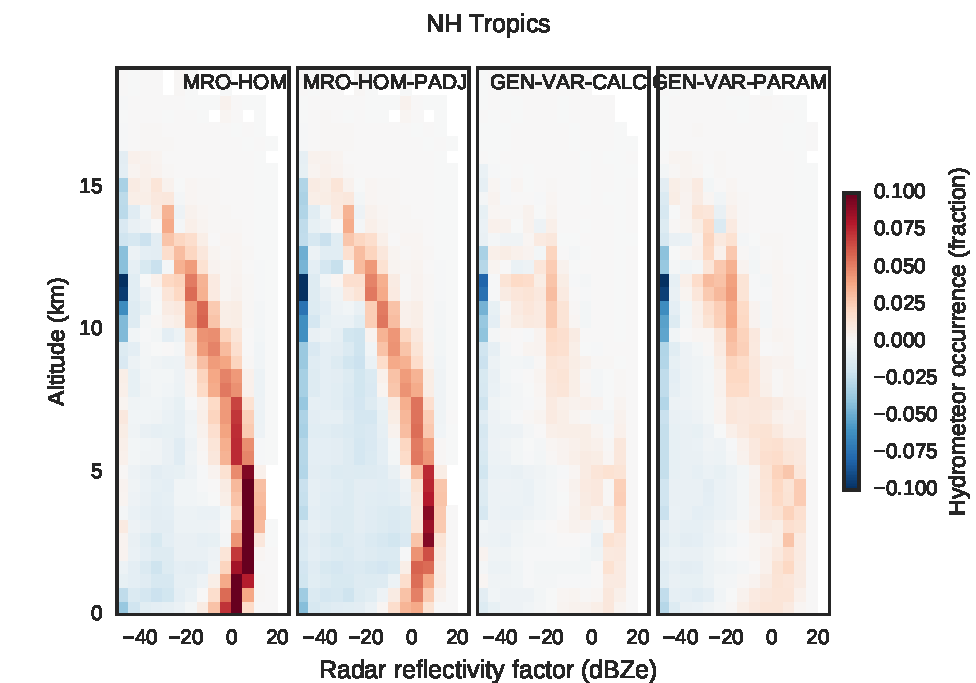
\includegraphics{graphics/subgrid2_cfadDbze94_NHTropics_all_diff.pdf}
\caption{\label{fig:subgrid2_cfadDbze94_NHTropics_all_diff}Errors in
CloudSat-simulated reflectivity with height histograms for the NH
Tropics (0 to 10 degrees
north).}\label{fig:subgrid2ux5fcfadDbze94ux5fNHTropicsux5fallux5fdiff}
\end{figure}

\section{Discussion}\label{sec:subgrid2Discussion}

In this chapter, a new cloud subcolumn generator using the algorithm of
\citet{raisanen_et_al_2004} has been presented to potentially replace
the current implementation of SCOPS in COSP. The new subcolumn generator
allows for a more realistic representation of cloud overlap by
representing overlap as a linear combination of maximum and random
overlap, as well as horizontally variable cloud and precipitation
condensate amount sampled from gamma distributions. The impact of these
changes on simulated satellite-observable cloud diagnostics from COSP
has been evaluated by using the new subcolumn generator to regenerate
subcolumns of cloud and precipitation condensate from CRM output from
SP-CAM that has been averaged to mimic gridbox mean quantities as would
be represented by a traditional GCM. These impacts have been tested both
with idealized overlap and horizontal variability calculated directly
from the original CRM fields and with overlap and horizontal variability
parameterized.

The ceiling of potential performance of the new subcolumn scheme is
demonstrated by running COSP on subcolumns regenerated with overlap and
variability calculated directly from the original CRM fields. It has
been shown here that this leads to substantial improvements in
satellite-simulated cloud properties. This suggests that implementing
this framework can substantially reduce errors in simulated clouds that
arise due to the currently used assumptions of maximum-random overlap
and horizontally homogeneous cloud and precipitation (as shown in the
previous chapter).

While results using the ideal (calculated) overlap and variability from
the original CRM fields demonstrate the potential of the new subcolumn
generator, results using the parameterized overlap and variability show
that the performance of the subcolumn generator is highly dependent on
how overlap and variability are parameterized within this framework. In
particular, it appears that MISR-simulated cloud area by cloud top
height is dependent on both the representation of variability and of
overlap, while CloudSat-simulated radar reflectivity is primarily
dependent on the representation of variability (and precipitation
occurrence, as demonstrated in the previous chapter). Large errors arise
when parameterizing overlap and rank correlation as functions of
separation distance alone with constant decorrelation length scales, and
it is shown that assuming constant decorrelation length scales is
insufficient for capturing the overlap characteristics of clouds
simulated by SP-CAM (see Figure~\ref{fig:subgrid2_overlap_maps} and
Figure~\ref{fig:subgrid2_rankcorr_maps}). However, substantially better
results are demonstrated when using decorrelation length scales that
depend on temperature, with separate (still spatially-invariant) scales
for warm and cold clouds, and overlap errors using the generalized
overlap treatment with overlap that depends on both the separation of
layers and on the temperature of the clouds results in a substantial
reduction of errors relative to those that arise using maximum-random
overlap.

Errors arising due to the parameterization of variability presented here
remain large for both MISR-simulated cloud area by cloud top height and
for CloudSat-simulated hydrometeor occurrence, but errors in
CloudSat-simulated reflectivity with height are still reduced somewhat
with even the crude parameterization of variability presented here. The
modest increase in performance from the improved treatment of
variability presented here, and the large increases in performance that
are possible as demonstrated using the calculated variability shows that
additional research is needed to better represent horizontal
subgrid-scale variability in large-scale models. These issues are not
unique to simulation of satellite-observable cloud diagnostics, and it
has been recognized that subgrid-scale variability, including cloud and
precipitation occurrence overlap and condensate amount, effect many
important processes in large-scale models, and some researchers are
trying to develop explicit subgrid treatments for GCMS. This includes
so-called ``statistical'' or ``assumed probability distribution''
schemes, which predict the evolution of not only the mean, but also the
probability distribution of total water (and hence the cloud and
precipitation condensate) within each grid-box
\citep[e.g.;][]{tompkins_2002}. There has been growing interest in using
these schemes in GCMs. One such example of this is the Cloud Layers
Unified By Binormals \citep[CLUBB;][]{golaz_et_al_2002} scheme, which is
being implemented into the NCAR CAM (A. Gettelman, personal
communication). Because these schemes explicitly assume a probability
distribution for the subgrid variability of condensate, they are a
natural fit to the stochastic treatment of subgrid clouds and
precipitation used in COSP to simulate satellite retrievals (and also to
radiation schemes that use stochastic treatments of subgrid clouds such
as the McICA \citep{pincus_et_al_2003}, because the same distribution of
condensate can be shared between these different components of the
model. As shown here for simulated satellite diagnostics and by others
for calculated radiative fluxes, these assumptions can have a large
impact on diagnosed cloud effects, and thus consistency between cloud
treatments in the different parts of the model is necessary in order to
obtain a consistent picture of the performance of models in simulating
clouds.
